\chapter{The supervised-learning contract}
\label{ch:supervised-contract}

\begin{learningobjectives}
After this chapter, you should be able to:
\begin{itemize}
  \item formulate a supervised-learning task as a statistical and operational contract;
  \item express learning through a hypothesis class, loss, population risk, and
  empirical procedure;
  \item derive the population targets selected by squared, absolute, and
  classification losses;
  \item distinguish features, targets, predictions, decisions, and causal claims;
  \item design a split that represents the intended prediction setting; and
  \item construct a baseline and a minimal training-to-feedback path.
\end{itemize}
\end{learningobjectives}

\begin{chapterconnection}
Chapter~\ref{ch:machine-learning-foundations} separated learning problems by
their information and feedback. We now specialize to labeled examples. Part I's
representation, package, database, API, and operational boundaries remain.
Supervised learning adds estimation error, a target-construction process,
adaptive selection, and a claim about transfer from observed labels to future
ones.
\end{chapterconnection}

\section{Supervised learning joins statistical inference and computation}

Long before the phrase machine learning, scientists estimated relationships
from paired measurements and tested rules on new observations. Twentieth-
century regression, discriminant analysis, experimental design, pattern
recognition, and statistical decision theory developed different parts of what
is now called supervised learning. Computing made it practical to search much
larger function classes, but it did not change the central question: what does a
finite labeled sample justify about a named population?

The modern abstraction is useful because it separates three objects. A
\term{model class} $\mathcal{F}$ contains candidate predictors. A
\term{learning rule} $\mathcal{A}$ maps labeled data $D$ to
$\widehat f_D\in\mathcal{F}$. A \term{prediction rule} applies the fitted
function to a new $x$. Confusing these objects leads to statements such as
``linear regression generalizes'' without identifying the sample, fitting
procedure, or future population.

\begin{misconceptionbox}
\textbf{Misconception:} supervised means that a human watches or corrects every
prediction. \textbf{Correction:} supervision refers to targets paired with
training inputs. Those targets may be delayed, noisy, algorithmically generated,
or institutionally defined; their presence does not make them ground truth.
\end{misconceptionbox}

\begin{warningbox}
A target can be measured consistently and still encode the wrong construct.
Historical approval, diagnosis, inspection, arrest, or hiring labels may reflect
prior access and policy as well as the underlying phenomenon. Supervision
transfers the target-generation process unless the design supplies evidence for
a stronger interpretation.
\end{warningbox}

\section{Learning begins with a future information boundary}

Let an observation be a pair $(X,Y)$ drawn from a population distribution
$P$. The feature vector $X\in\mathcal{X}$ contains information available at a
specified prediction time. The target $Y\in\mathcal{Y}$ records the outcome to
be estimated. A learning algorithm receives a sample
$D=\{(x_i,y_i)\}_{i=1}^n$ and produces a predictor
$\widehat f_D:\mathcal{X}\rightarrow\mathcal{A}$. The action space
$\mathcal{A}$ may contain numerical estimates, scores, probabilities, or class
labels.

This notation is compact enough to hide the most important design decisions.
What is one observational unit? From which population were units sampled? At
what time is $X$ frozen? How far in the future is $Y$ measured? Which units can
recur? What action consumes the output? The subscript $D$ is a reminder that a
fitted predictor is random: a different sample can produce a different
function.

\begin{definitionbox}{supervised-learning contract}
A supervised-learning contract names the observational unit, target population,
prediction time, target and horizon, permitted information, output semantics,
loss or utility, evaluation design, operational consumer, and outcome-feedback
process. The model class is one field in this contract, not the contract itself.
\end{definitionbox}

Our recurring case concerns battery cells. At the end of an early measurement
window, we may estimate capacity after a later number of cycles, or predict
whether the cell will cross a degradation threshold within a stated horizon.
Measurements collected after the prediction time are forbidden, even if they
appear in the same convenient table.

\section{Risk, empirical risk, and the generalization claim}

For a loss function $L(y,a)$, the population risk of $f$ is
\[
R(f)=\mathbb{E}_{(X,Y)\sim P}[L(Y,f(X))].
\]
The distribution $P$ is generally unknown. Training therefore uses an empirical
quantity such as
\[
\widehat R_D(f)=\frac{1}{n}\sum_{i=1}^n L(y_i,f(x_i)).
\]
Minimizing empirical loss is a computational objective. The scientific claim
is that performance transfers to a named population and use setting. That claim
depends on sampling, dependence, temporal stability, measurement, and the way
the model was selected.

A loss trains or compares functions. A metric communicates some aspect of
behavior. A decision policy converts output into action. These objects can be
different. Logistic loss may fit a probability model, calibration error may
audit its probabilities, and an asymmetric cost rule may choose an intervention
threshold.

Regularized empirical risk minimization makes the preference explicit:
\[
\widehat f\in\arg\min_{f\in\mathcal{F}}
\left\{\widehat R_D(f)+\lambda\Omega(f)\right\}.
\]
Here $\Omega$ may penalize coefficient size, roughness, tree complexity, or
another property. The value $\lambda$ is selected using development data, not
the final test set. Restricting $\mathcal{F}$ and penalizing within
$\mathcal{F}$ are both forms of inductive bias.

\section{The loss determines the population target}

Suppose predictors may choose any real number $a$ at a fixed $X=x$. The loss
does not merely grade a prediction after training; it defines which population
functional an unrestricted learner attempts to estimate.

\begin{theorem}[Squared loss elicits the conditional mean]
\label{thm:squared-loss-mean}
Assume $\mathbb{E}[Y^2\mid X=x]<\infty$ and write
$\mu(x)=\mathbb{E}[Y\mid X=x]$. The conditional squared-error risk
\[
q(a)=\mathbb{E}[(Y-a)^2\mid X=x]
\]
is uniquely minimized at $a=\mu(x)$.
\end{theorem}

\begin{proof}
Add and subtract $\mu=\mu(x)$, expand, and condition on $X=x$:
\begin{align*}
q(a)
&=\mathbb{E}[(Y-\mu+\mu-a)^2\mid X=x]\\
&=\mathbb{E}[(Y-\mu)^2\mid X=x]
  +2(\mu-a)\mathbb{E}[Y-\mu\mid X=x]+(\mu-a)^2\\
&=\operatorname{Var}(Y\mid X=x)+(\mu-a)^2.
\end{align*}
The first term does not depend on $a$ and the second is nonnegative, with
equality only at $a=\mu$. This argument avoids assuming a density or
differentiating through an expectation.
\end{proof}

Under absolute loss, $\mathbb{E}[|Y-a|\mid X=x]$ is minimized by a conditional
median. Under binary zero-one loss, the most probable class minimizes
conditional error. Quantile loss targets a conditional quantile. Thus two
teams can use the same rows and model family yet estimate different population
objects because their losses differ.

These are mathematical targets, not interchangeable metrics. If a laboratory
needs a high conditional quantile to plan safety stock, fitting a conditional
mean answers the wrong question even if the optimizer is perfect.

For binary action $d\in\{0,1\}$ with false-positive cost $C_{FP}$ and
false-negative cost $C_{FN}$, the Bayes action compares conditional expected
costs. With a calibrated probability $p(x)=P(Y=1\mid X=x)$ and no other
constraints, act when
\[
C_{FP}[1-p(x)]<C_{FN}p(x).
\]
Thus the model output and the decision threshold solve related but distinct
problems.

\conceptcheck{At a fixed feature vector, the conditional distribution of $Y$
is strongly right-skewed. Which population summaries are targeted by squared
and absolute loss? Why might the two fitted predictions differ even with
infinite representative data?}

\section{Generalization error has several sources}

Let $f^*$ minimize risk over all measurable predictors and let
$f^*_{\mathcal{F}}$ minimize risk within $\mathcal{F}$. The excess risk can be
organized conceptually as
\[
R(\widehat f_D)-R(f^*)
=\underbrace{R(f^*_{\mathcal{F}})-R(f^*)}_{\text{approximation}}
+\underbrace{R(\widehat f_D)-R(f^*_{\mathcal{F}})}_{\text{estimation and optimization}}.
\]
The second term combines finite-sample variation with any failure to solve the
fitting problem. Distribution shift adds another discrepancy because the
evaluation population may no longer match training.

For squared-error regression at a fixed $x$, averaging over possible training
samples yields the familiar bias-variance decomposition
\[
\mathbb{E}_{D,Y\mid x}[(Y-\widehat f_D(x))^2]
=\sigma^2(x)
+\left(\mathbb{E}_D[\widehat f_D(x)]-f(x)\right)^2
+\operatorname{Var}_D(\widehat f_D(x)),
\]
when $f(x)=\mathbb{E}[Y\mid X=x]$ and
$\sigma^2(x)=\operatorname{Var}(Y\mid X=x)$. Irreducible outcome variation,
systematic estimator bias, and sample-to-sample instability are different
phenomena. A single fitted dataset cannot display the decomposition directly;
resampling and scientific replication provide evidence about stability.

\conceptcheck{A laboratory reports excellent mean squared error after randomly
splitting rows, but each physical cell contributes many rows to both subsets.
What population quantity does that experiment estimate, and why might it differ
from performance on a previously unseen cell?}

\section{Prediction is not causal explanation}

A predictor exploits associations that persist between its training and use
settings. It need not represent a mechanism. A variable can improve prediction
because it is a proxy for laboratory, instrument, treatment assignment, or
selection process. Conversely, a causally important variable may add little
predictive information if its variation is small or already encoded elsewhere.

The question ``What will happen?'' differs from ``What would happen if we
intervened?'' Counterfactual conclusions require additional design and
assumptions. High predictive accuracy does not supply them.

\begin{misconceptionbox}
\textbf{Misconception:} a sufficiently accurate model discovers the true
causes. \textbf{Correction:} predictive performance is evidence about a
specified prediction task under a specified evaluation design. Causal claims
require an identification argument that predictive accuracy alone cannot
provide.
\end{misconceptionbox}

\section{Splits simulate the use setting}

A random row split is appropriate only when future uses resemble independent
draws from the same row-level population. Dependence changes the unit of
separation. Repeated measures from one cell call for grouped splitting when the
claim concerns unseen cells. Forecasting calls for training on the past and
evaluating on the future. A new laboratory or manufacturing batch may require a
held-out domain.

Three subsets have different responsibilities. Training data determine fitted
parameters. Validation data guide model and hyperparameter choices. Test data
support a final estimate after those choices stop. Cross-validation rotates
training and validation roles; it does not excuse repeatedly consulting the
test set.

\begin{theorem}[What an independent test average estimates]
\label{thm:test-risk-unbiased}
Condition on a completed training and selection process that produces a fixed
predictor $\widehat f$. If test pairs $(X_j,Y_j)$ are independent draws from
$P_{\mathrm{use}}$ and are independent of that process, then
\[
\widehat R_{\mathrm{test}}(\widehat f)
=\frac1m\sum_{j=1}^{m}L(Y_j,\widehat f(X_j))
\]
is conditionally unbiased for $R(\widehat f)$.
\end{theorem}

\begin{proof}
Conditional on $\widehat f$, linearity of expectation and identical sampling
give
\[
\mathbb{E}[\widehat R_{\mathrm{test}}(\widehat f)\mid\widehat f]
=\frac1m\sum_{j=1}^{m}
\mathbb{E}_{P_{\mathrm{use}}}[L(Y,\widehat f(X))]
=R(\widehat f).
\]
The conclusion fails when test observations influence feature construction,
model choice, stopping, or repeated reporting. In that case $\widehat f$ is no
longer fixed independently of the claimed test evidence.
\end{proof}

\term{Leakage} occurs when model construction uses information that would not
be legitimately available at prediction time or crosses an evaluation
boundary. Target-derived features are obvious leakage. More subtle cases
include fitting normalization on the full dataset, selecting variables before
cross-validation, using future measurements, and allowing related entities into
both sides of a split.

\begin{warningbox}
Preprocessing learns parameters too. Imputation values, category vocabularies,
scales, feature selection, and representation learning must be fitted using the
training portion of each evaluation fold and then applied to held-out data.
\end{warningbox}

Figure~\ref{fig:supervised-evidence} shows the three roles on the real diabetes
table. Polynomial degree is varied only against validation data. The sealed
test subset is then used once to compare the selected candidate with a baseline.
The particular winning degree is not a scientific conclusion; it is a concrete
demonstration of information flow.

\begin{figure}[htbp]
  \centering
  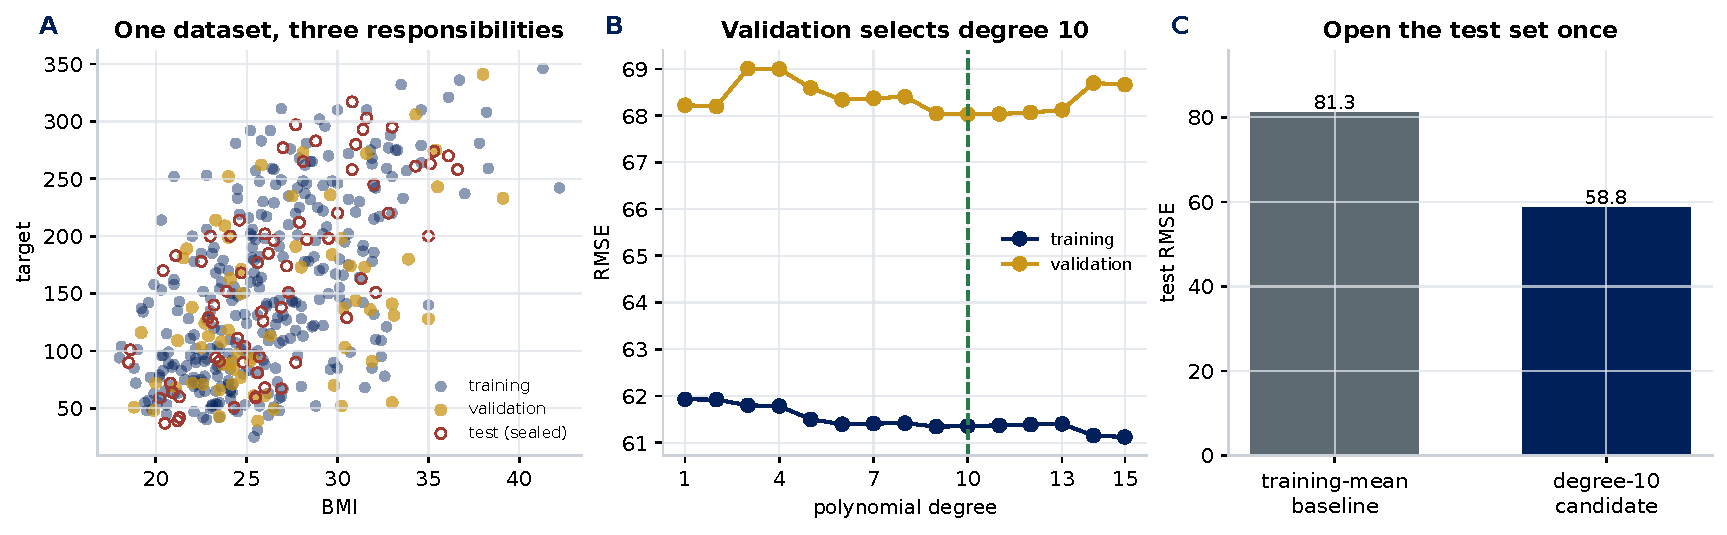
\includegraphics[width=\textwidth]{figures/generated/supervised-evidence.pdf}
  \caption{Training estimates parameters, validation supports adaptive choices,
  and test data estimate the performance of the completed procedure. Re-running
  model selection after viewing panel C would turn the test set into development
  data.}
  \label{fig:supervised-evidence}
\end{figure}

\section{A baseline is an experimental control}

A baseline asks whether learning adds value beyond a simple policy. For
regression, predict the training mean or a physically motivated constant. For
classification, predict class prevalence or the most frequent class, but audit
whether that behavior is useful under imbalance. A time-series baseline may
carry the latest observation forward.

The baseline uses the same split, metric, and information boundary as the
candidate. Otherwise it is not a control. A complex model that fails to beat a
correct baseline has supplied diagnostic evidence: the signal, representation,
sample size, objective, or implementation may not support the claim.

\section{Measure predictive performance as an experiment}

For regression residuals $e_i=y_i-\widehat y_i$, three common summaries are
\[
\operatorname{MAE}=\frac1m\sum_{i=1}^m|e_i|,
\qquad
\operatorname{RMSE}=\sqrt{\frac1m\sum_{i=1}^m e_i^2},
\]
and
\[
R^2=1-\frac{\sum_i e_i^2}{\sum_i(y_i-\bar y)^2}.
\]
MAE retains the target unit and weights errors linearly. RMSE has the target
unit but emphasizes large residuals. $R^2$ compares squared error with the
constant test-set mean benchmark; it is not a percentage of predictions that
are correct, and it can be negative on held-out data. Always report the unit,
sample count, and reference policy beside the number.

A metric estimate also has sampling variation. If evaluation units are
independent, a bootstrap that resamples those units can describe uncertainty.
If measurements are grouped by patient, machine, site, or time block, resample
the independent group instead of individual rows. The resampling unit must
match the generalization claim. For paired model comparison, compute both
models on the same units and resample their per-unit loss differences; this
retains the information that an observation was easy or difficult for both.

Predictive quality is only one budget. Record fit time separately from
prediction time, and measure prediction latency at representative batch sizes.
Report a tail quantile such as the 95th or 99th percentile when a service-level
objective concerns slow requests. Measure peak memory for training and serving
independently. A model with slightly lower RMSE may be dominated if it violates
the latency, memory, interpretability, or outcome-feedback requirements stated
in the supervised-learning contract.

\begin{professionalbox}
Store evaluation as a table with one row per evaluation unit: identifiers,
observed target, prediction, model version, subgroup fields permitted for audit,
and per-unit loss. Aggregate reports can then be reproduced, sliced, paired,
and bootstrapped. A screenshot of one score is not durable evaluation evidence.
\end{professionalbox}

\section{One table can contain many supervised problems}

Application design determines the unit, target, horizon, and split.

\begin{tabularx}{\textwidth}{@{}>{\raggedright\arraybackslash}p{0.17\textwidth}>{\raggedright\arraybackslash}p{0.26\textwidth}>{\raggedright\arraybackslash}X@{}}
\toprule
Application & Supervised target & Evaluation boundary \\
\midrule
Materials & Capacity after 300 cycles from the first 100 cycles & Hold out
cells and later manufacturing batches \\
Public health & Next-week regional case count from reports available today &
Train on past weeks and preserve reporting-delay behavior \\
Remote sensing & Land-cover class from multispectral pixels & Hold out spatial
regions or acquisition campaigns, not random neighboring pixels \\
Predictive maintenance & Failure within 30 operating days from sensor history
& Separate machines and respect the feature cutoff before failure \\
Scientific literature & Relevance of a paper to a review protocol & Preserve
reviewer disagreement and evaluate on later searches \\
\bottomrule
\end{tabularx}

Random splitting would answer a different and often easier question in every
row. The split is part of the estimand: it defines the population transfer the
reported metric attempts to approximate.

\begin{workedexample}{write the battery prediction contract}
Suppose one row summarizes the first 100 cycles of one cell. The target is
capacity at cycle 300, measured in ampere-hours. The intended use is prediction
for cells from future manufacturing batches immediately after cycle 100.

The feature cutoff excludes all observations after cycle 100. Batch identity
defines an outer temporal split: earlier batches train the system and later
batches evaluate it. All transformations are fitted within the training side.
The baseline predicts the mean training capacity at cycle 300. Mean absolute
error is reported in ampere-hours together with the error distribution by batch.

The contract also states what it does not establish. It does not estimate the
effect of changing a charging protocol, certify safety, or guarantee behavior
for a chemistry absent from the study. Those exclusions are part of the result,
not fine print.
\end{workedexample}

\section{The first vertical slice should be deliberately simple}

Before optimizing an algorithm, prove that the system can reproduce a split,
fit a baseline, serialize an artifact, load it in a separate process, validate
inputs, produce predictions, record model and feature versions, and later join
predictions to outcomes. A dummy model is ideal because unexpected behavior is
easy to detect.

The artifact manifest should identify training data, code revision,
configuration, feature schema, split policy, fitted object, evaluation report,
and creation time. A model file without this context is an opaque binary, not a
reproducible result.

\section{Exercises}

Use the printed identifier when discussing, submitting, or contributing a
problem. A repository contribution follows the issue-to-PR procedure in
Appendix~\ref{app:git-github}; the mathematics remains part of its review
contract.

\subsection*{Intuition and explanation}

\begin{enumerate}[label=\textbf{SLC-I\arabic*.},leftmargin=*,itemsep=0.65em]
  \item Write two prediction contracts for the same battery table: one for an
  unseen cell from a known batch and one for a cell from a future batch. Explain
  why their splits, plausible shifts, and release claims differ.
  \item Give temporal, group, preprocessing, and target-construction leakage
  examples. For each, draw the forbidden information path and explain why a
  high held-out score may survive the mistake.
  \item A label is measured reproducibly but reflects an earlier institution's
  decision policy. Explain what a predictor of that label learns, what it does
  not learn, and which additional evidence would justify the intended construct.
  \item Distinguish loss, evaluation metric, calibrated score, and decision
  policy using one high-stakes classification example.
\end{enumerate}

\subsection*{Mathematical reasoning}

\begin{enumerate}[label=\textbf{SLC-M\arabic*.},leftmargin=*,itemsep=0.65em]
  \item Re-prove Theorem~\ref{thm:squared-loss-mean} by differentiating the
  conditional risk, and list the regularity assumptions your proof uses. Compare
  them with the completion-of-squares proof in the chapter.
  \item Prove that every conditional median minimizes conditional absolute
  loss. Treat nonunique medians carefully by using one-sided derivatives or a
  direct comparison of integrals.
  \item Under the assumptions of Theorem~\ref{thm:test-risk-unbiased}, derive
  $\operatorname{Var}(\widehat R_{\mathrm{test}}\mid\widehat f)$. Explain how
  dependence among repeated measurements changes the result.
  \item Derive the cost-sensitive binary threshold
  $C_{FP}/(C_{FP}+C_{FN})$ from conditional expected cost. Give two operational
  constraints that make this threshold incomplete.
  \item For squared error, derive the fixed-$x$ bias-variance decomposition.
  Identify which expectation is over future outcomes and which is over possible
  training samples.
\end{enumerate}

\subsection*{Data and engineering investigations}

\begin{enumerate}[label=\textbf{SLC-C\arabic*.},leftmargin=*,itemsep=0.65em]
  \item Recreate Figure~\ref{fig:supervised-evidence} with five different split
  seeds. Report how often each polynomial degree is selected and what this says
  about treating one validation winner as a scientific discovery.
  \item Build a leakage-safe baseline and candidate pipeline for one course
  table. Preserve one row per evaluation unit with target, prediction, residual,
  model version, and permitted audit fields. Report MAE, RMSE, $R^2$, a paired
  comparison, and the limitations of the split.
  \item Measure prediction latency at batch sizes 1, 16, and 256 after warmup.
  Record hardware, dependency lock, repetitions, median, 95th percentile, and
  whether preprocessing is included. Explain which result matters for an API
  and which for an offline batch job.
  \item Design and test an artifact manifest that rejects reordered, missing,
  duplicated, or unit-incompatible inputs before inference.
\end{enumerate}

\subsection*{Contribution studio}

Choose one scoped addition and preserve the problem identifier from issue
through merge.

\begin{enumerate}[label=\textbf{SLC-PR\arabic*.},leftmargin=*,itemsep=0.65em]
  \item Add a typed prediction-contract component with validation for unit,
  population, feature cutoff, horizon, target, split policy, metric, consumer,
  and feedback delay. Include round-trip serialization and failure tests.
  \item Add a reusable paired regression report that accepts observed values
  and two prediction vectors, returns per-unit losses and aggregate differences,
  and never silently drops nonfinite or misaligned values.
  \item Add a custom split validator for a domain you choose--grouped,
  temporal, spatial, or batch-based. Document the claim it protects, construct
  an adversarial leakage fixture, and test that the invalid split is rejected.
\end{enumerate}

\begin{chapterreview}
Supervised learning estimates a rule from paired inputs and targets, but the
defensible object is larger than the fitted rule. A loss defines a population
target; a hypothesis class and regularizer encode inductive bias; a learning
rule introduces estimation and optimization behavior. The contract names
population, time, target, information, split, consumer, and feedback.
Evaluation must simulate intended use, baselines act as controls, and the first
vertical slice should validate artifact and evidence flow before model
complexity grows. Metrics require units, uncertainty, a reference policy, and a
resource-aware measurement protocol.
\end{chapterreview}

\begin{notebooklink}
Lecture 9 notebook 01 begins by writing the supervised contract for a real
diabetes-progression dataset. It separates training, validation, and test roles,
derives the squared-loss target, fits baselines, and constructs preprocessing
inside the training boundary. Its clinical example is a methods laboratory,
not a deployment claim; missing site, time, and patient identifiers are treated
as limitations rather than silently ignored.
\end{notebooklink}
